\documentclass[12pt,letterpaper]{article}

\usepackage{assignments}
% \usepackage{minted}
\usepackage{graphicx}
\usepackage{bm}
\usepackage{amsmath}
\usepackage{amssymb}
\usepackage{subcaption}

\begin{document}

\title{\vspace{-4ex}ECE521: Inference Algorithms and Machine Learning \\
University of Toronto\\ \  \\
Solution to Assignment 3: \\Unsupervised Learning and Probabilistic Models}
\author{Renjie Liao}
% \date{\vspace{-8ex}TA: Use Piazza for Q\&A \\ Due date: Mar. 24 11:59 pm, 2017 \\ Electronic submission to: \href{mailto:ece521ta@gmail.com}{ece521ta@gmail.com} }


\maketitle

\begin{mycomments}
\section{Part 1}
\end{mycomments}
\section{K-means}

\subsection{Learning K-means [8 pt.]}

1, [3 pt.] The loss function $\mathcal{L}(\bm{\mu})$ is non-convex in $\bm{\mu}$. We use contradiction to prove the statement. Assuming $\mathcal{L}(\bm{\mu})$ is convex in $\bm{\mu}$. 
We consider a special case where $B = 1$, $K = 2$, $D = 2$, $\mathbf{x} = \left[x_1, x_2\right]$, $\mathbf{\bm{\mu}} = \left[\bm{\mu}_1, \bm{\mu}_2\right]$ and $\mathbf{x} \neq \mathbf{0}$. 
We can rewrite the loss function as $\mathcal{L}(\bm{\mu}) = \min(\Vert \mathbf{x} - \bm{\mu}_{1} \Vert_{2}^{2}, \Vert \mathbf{x} - \bm{\mu}_{2} \Vert_{2}^{2})$. 
Now we will show that for two specific constructions $\mathbf{\bm{\mu}} = \left[\bm{\mu}_1, \bm{\mu}_2\right]$ and $\mathbf{\bm{\mu}^{\prime}} = \left[\bm{\mu}_{1}^{\prime}, \bm{\mu}_{2}^{\prime}\right]$ and any $\theta \in (0, 1)$, we have $\mathcal{L}(\theta \bm{\mu} + (1 - \theta) \bm{\mu}^{\prime}) > \theta \mathcal{L}(\bm{\mu}) + (1 - \theta) \mathcal{L}(\bm{\mu}^{\prime})$. 
In particular, let $\bm{\mu}_{1} = \left[ x_{1}, x_{2} \right]$, $\bm{\mu}_{2} = \left[ 0, 0 \right]$, $\bm{\mu}_{1}^{\prime} = \left[ 0, 0 \right]$ and $\bm{\mu}_{2}^{\prime} = \left[ x_{1}, x_{2} \right]$. 
We have that $\mathcal{L}(\bm{\mu}) = 0$ and $\mathcal{L}(\bm{\mu}^{\prime}) = 0$. 
Moreover, we have,
\begin{align}
\mathcal{L}(\theta \bm{\mu} + (1 - \theta) \bm{\mu}^{\prime}) & = \min(\Vert \mathbf{x} - \theta \bm{\mu}_{1} - (1 - \theta) \bm{\mu}_{1}^{\prime} \Vert_{2}^{2}, \Vert \mathbf{x} - \theta \bm{\mu}_{2} - (1 - \theta) \bm{\mu}_{2}^{\prime} \Vert_{2}^{2}) \nonumber \\
& = \min( (1 - \theta)^{2} \Vert \mathbf{x} \Vert^{2}, \theta^{2} \Vert \mathbf{x} \Vert^{2} ).
\label{kmeans_ineq}
\end{align}
It is thus clear that $\mathcal{L}(\theta \bm{\mu} + (1 - \theta) \bm{\mu}^{\prime}) > \theta \mathcal{L}(\bm{\mu}) + (1 - \theta) \mathcal{L}(\bm{\mu}^{\prime}) = 0$ for any $\theta \in (0, 1)$. Hence, we have the contradiction.

\begin{figure}
    \centering
    \begin{subfigure}[b]{0.45\textwidth}
        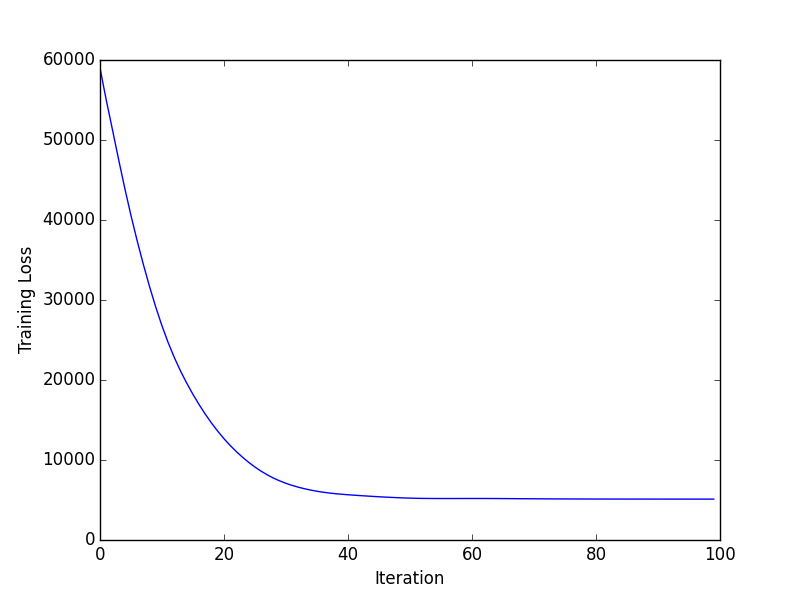
\includegraphics[width=\textwidth]{imgs/kmeans_train_loss.png}
        \caption{Kmeans, training loss}
        \label{kmeans_loss}
    \end{subfigure}
    \begin{subfigure}[b]{0.45\textwidth}
        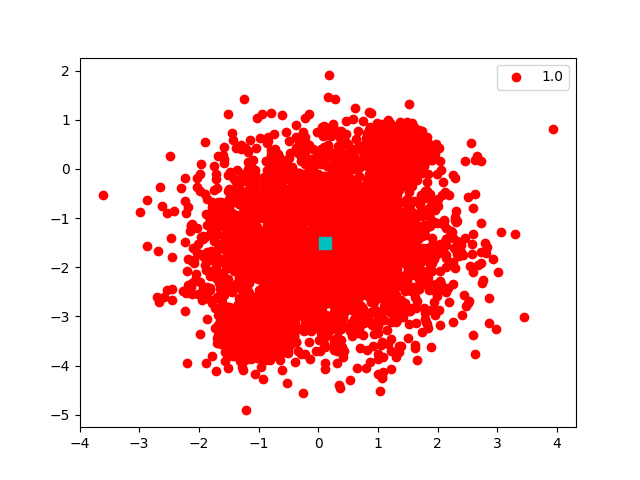
\includegraphics[width=\textwidth]{imgs/kmeans_K_1.png}
        \caption{Kmeans, K = 1}
        \label{kmeans_1}
    \end{subfigure}

    \begin{subfigure}[b]{0.45\textwidth}
        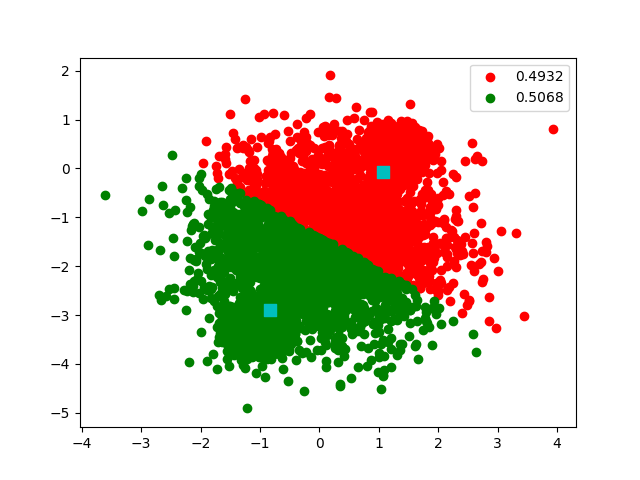
\includegraphics[width=\textwidth]{imgs/kmeans_K_2.png}
        \caption{Kmeans, K = 2}
        \label{kmeans_2}
    \end{subfigure}
    \begin{subfigure}[b]{0.45\textwidth}
        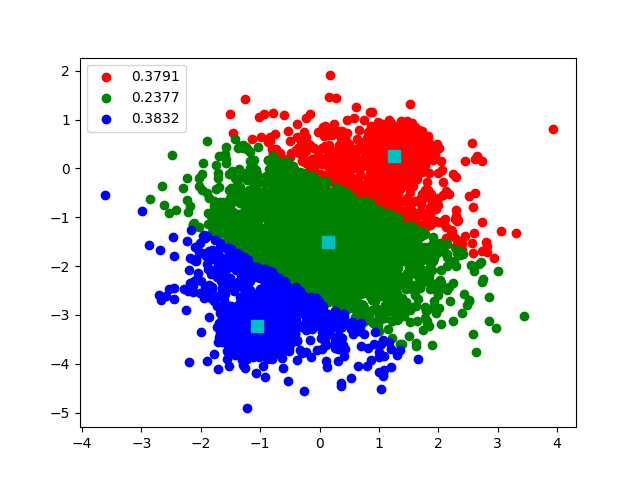
\includegraphics[width=\textwidth]{imgs/kmeans_K_3.png}
        \caption{Kmeans, K = 3}
        \label{kmeans_3}
    \end{subfigure}
     
    %add desired spacing between images, e. g. ~, \quad, \qquad, \hfill etc. 
    %(or a blank line to force the subfigure onto a new line)
    \begin{subfigure}[b]{0.45\textwidth}
        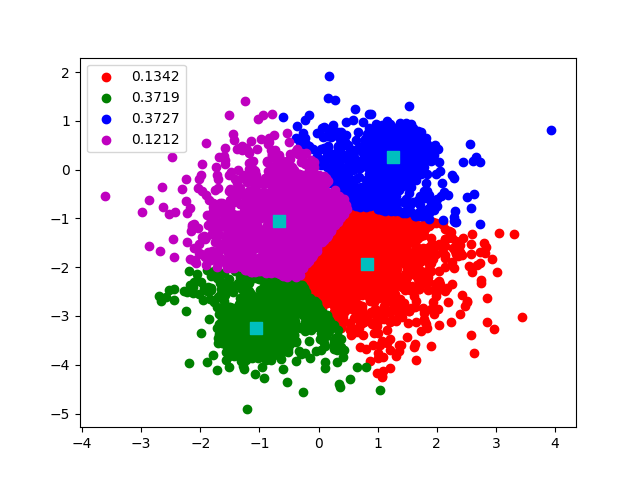
\includegraphics[width=\textwidth]{imgs/kmeans_K_4.png}
        \caption{Kmeans, K = 4}
        \label{kmeans_4}
    \end{subfigure}
    \begin{subfigure}[b]{0.45\textwidth}
        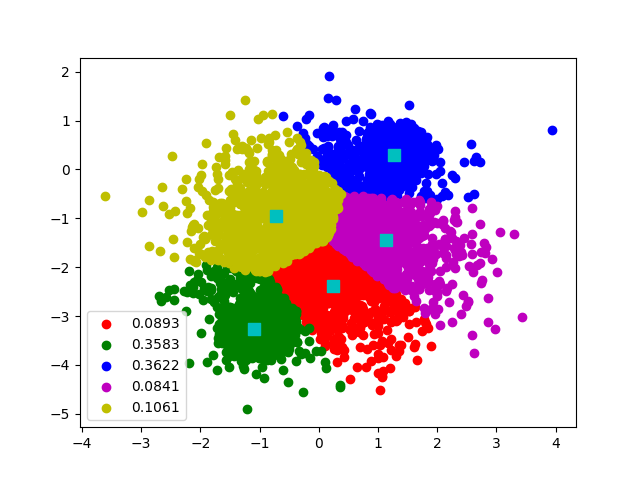
\includegraphics[width=\textwidth]{imgs/kmeans_K_5.png}
        \caption{Kmeans, K = 5}
        \label{kmeans_5}
    \end{subfigure}
\end{figure}


2, [2 pt.] Referring to Fig. \ref{kmeans_loss}.

3, [3 pt.] Referring to Fig. \ref{kmeans_1} - \ref{kmeans_5}. K = 5 might be the best as it gives the lowest loss function value.

4, [2 pt.] The validation loss values are $12856.2089844$, $2982.43554688$, $1659.61975098$, $1095.4954834$, $921.618164062$ when $K = 1, 2, 3, 4, 5$ respectively. Therefore, $K = 5$ is the best.


\section{Mixtures of Gaussians}

\subsection{The Gaussian cluster model}

1, [3 pt.] 
\begin{align}
P(z | \mathbf{x}) = \frac{ \pi^{k} \left( \sigma^{k} \right)^{-D} \exp \left\{ -\frac{1}{2 \left( \sigma^{k} \right)^{2}} (\mathbf{x} - \bm{\mu}^{k})^{\top} (\mathbf{x} - \bm{\mu}^{k}) \right\} }{ \sum_{j=1}^{K} \pi^{j} \left( \sigma^{j} \right)^{-D} \exp \left\{ -\frac{1}{2 \left( \sigma^{j} \right)^{2}} (\mathbf{x} - \bm{\mu}^{j})^{\top} (\mathbf{x} - \bm{\mu}^{j}) \right\} }
\label{GMM_posterior}
\end{align}

2, [2 pt.] Referring to Fig. \ref{dist_func}.
\begin{figure}
\centering
    \begin{subfigure}[b]{0.45\textwidth}
        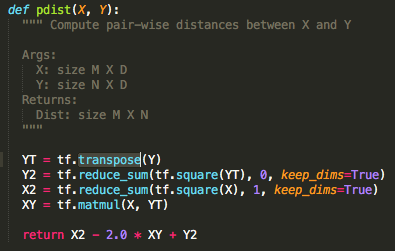
\includegraphics[width=\textwidth]{imgs/GMM_2_1_2.png}
        \caption{Distance function.}
        \label{dist_func}
    \end{subfigure}
    \begin{subfigure}[b]{0.45\textwidth}
        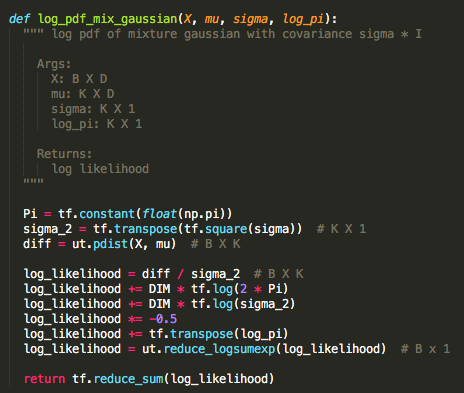
\includegraphics[width=\textwidth]{imgs/GMM_2_1_3.png}
        \caption{Log probability.}
        \label{log_prob}
    \end{subfigure}
\end{figure}

3, [3 pt.] Referring to Fig. \ref{log_prob}. Using log-sum-exp is numerically more accurate and stable and will help avoid issues like underflow or overflow.

\subsection{Learning the MoG}

1, [2 pt.]
\begin{align}
\nabla_{\bm{\mu}} \log P(\mathbf{x}) & = \nabla_{\bm{\mu}} \log \left( \sum_{k=1}^{K} P(\mathbf{x}, z=k) \right) \nonumber \\
& = \frac{1}{\sum_{k=1}^{K} P(\mathbf{x}, z=k)} \sum_{k=1}^{K} \nabla_{\bm{\mu}} P(\mathbf{x}, z=k) \nonumber \\
& = \frac{1}{\sum_{k=1}^{K} P(\mathbf{x}, z=k)} \sum_{k=1}^{K} P(\mathbf{x}, z=k) \nabla_{\bm{\mu}} \log P(\mathbf{x}, z=k) \nonumber \\
& = \sum_{k=1}^{K} P(z=k | \mathbf{x}) \nabla_{\bm{\mu}} \log P(\mathbf{x}, z=k),
\label{GMM_posterior}
\end{align}
where we use the fact $f(x) \nabla_x \log (f(x)) = \nabla_x f(x)$.

2, [6 pt.] Referring to Fig. \ref{GMM_loss}. The best model parameters are: $\mu_1 = [-1.09925008 -3.30307055]$, $\mu_2 = [1.29940867  0.30630079]$, $\mu_1 = [0.09809401 -1.5353744]$, $\sigma_1 = 0.19823763$, $\sigma_2 = 0.19667165$, $\sigma_3 = 0.99854809$, $\pi_1 = 0.32968238$, $\pi_2 = 0.33281365$ and $\pi_3 = 0.33750394$.

\begin{figure}
    \centering
    \begin{subfigure}[b]{0.45\textwidth}
        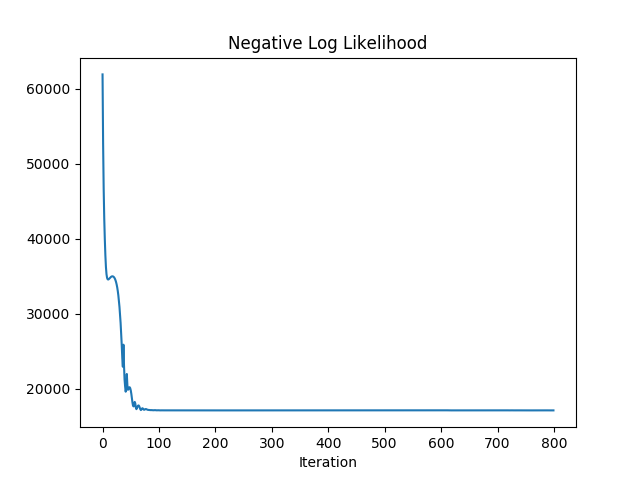
\includegraphics[width=\textwidth]{imgs/gmm_train_loss.png}
        \caption{GMM training loss}
        \label{GMM_loss}
    \end{subfigure}
    \begin{subfigure}[b]{0.45\textwidth}
        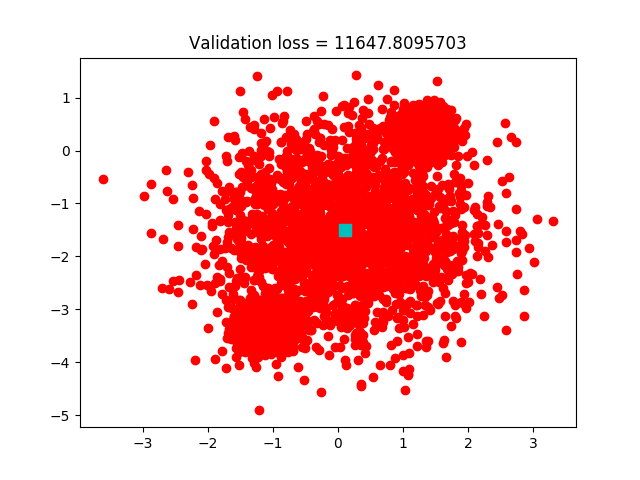
\includegraphics[width=\textwidth]{imgs/GMM_K_1.png}
        \caption{GMM, K = 1}
        \label{GMM_1}
    \end{subfigure}

    \begin{subfigure}[b]{0.45\textwidth}
        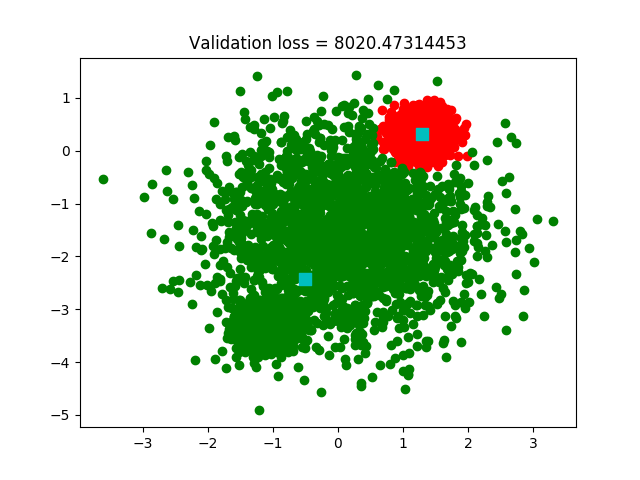
\includegraphics[width=\textwidth]{imgs/GMM_K_2.png}
        \caption{GMM, K = 2}
        \label{GMM_2}
    \end{subfigure}
    \begin{subfigure}[b]{0.45\textwidth}
        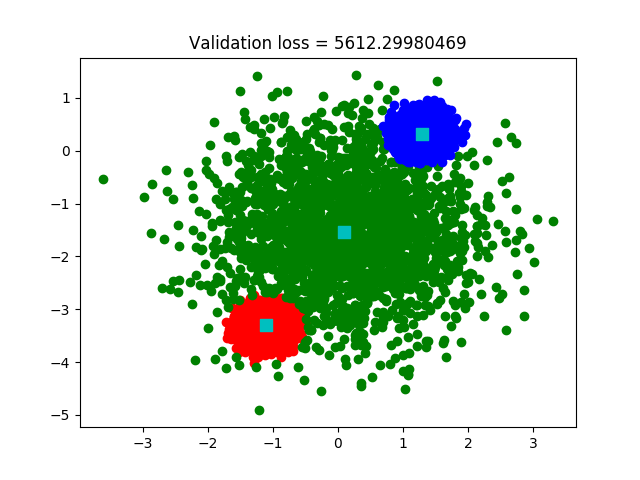
\includegraphics[width=\textwidth]{imgs/GMM_K_3.png}
        \caption{GMM, K = 3}
        \label{GMM_3}
    \end{subfigure}
     
    %add desired spacing between images, e. g. ~, \quad, \qquad, \hfill etc. 
    %(or a blank line to force the subfigure onto a new line)
    \begin{subfigure}[b]{0.45\textwidth}
        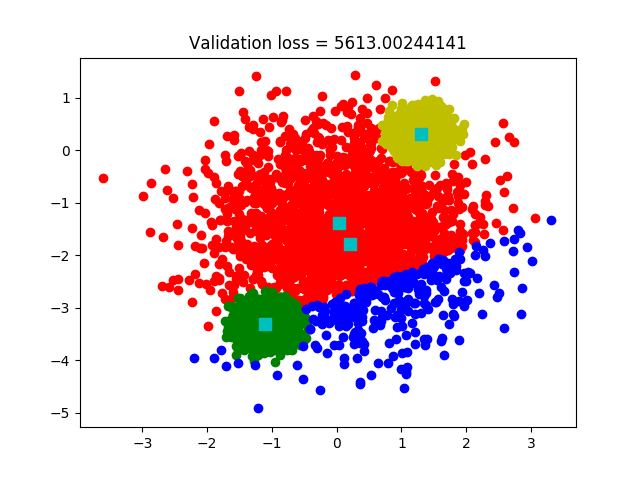
\includegraphics[width=\textwidth]{imgs/GMM_K_4.png}
        \caption{GMM, K = 4}
        \label{GMM_4}
    \end{subfigure}
    \begin{subfigure}[b]{0.45\textwidth}
        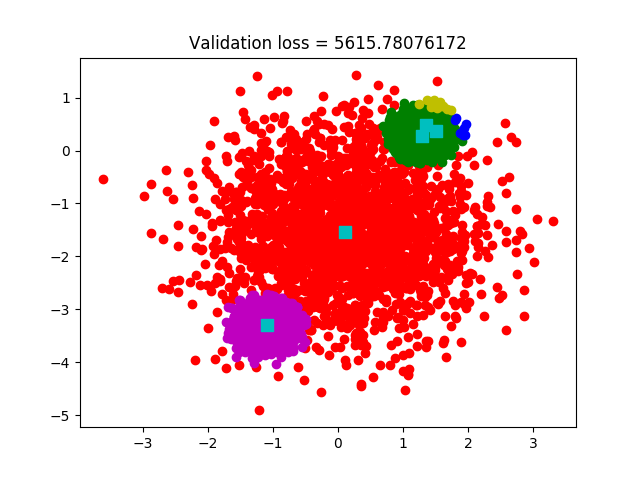
\includegraphics[width=\textwidth]{imgs/GMM_K_5.png}
        \caption{GMM, K = 5}
        \label{GMM_5}
    \end{subfigure}
\end{figure}

3, [2 pt.] Referring to Fig. \ref{GMM_1} - \ref{GMM_5}. $K = 3$ is the best as the validation loss is the minimum.

4, [2 pt.] The loss function values of Kmeans and MoG with different K are listed in the table \ref{loss_table}. From the current trials, it seems that the number of clusters should be around 20. We visualize the cluster assignments and cluster centers in terms of the first 2 dimensions of the 100D dataset in Fig. \ref{kmeans_100D} and Fig. \ref{GMM_100D}. It is hard to draw any conclusion from the learned results. It seems that some clusters of GMM are collapsed while the ones of Kmeans are not.

\begin{table}
\centering
\begin{tabular}{ l | c c }
& GMM & Kmeans \\ \hline
k=3 & 651434.875 & 1418950.625 \\ \hline
k=5 & 352855.46875 & 1091327.0 \\ \hline
k=10 & 211011.671875 & 1304746.25 \\ \hline
k=15 & 209351.46875 & 486612.15625 \\ \hline
k=20 & 207494.59375 & 484491.625 \\ \hline
k=30 & 204230.015625 & 485255.78125
\end{tabular}
\caption{Loss values on 100D dataset.}
\label{loss_table}
\end{table}

\begin{figure}
    \centering
    \begin{subfigure}[b]{0.45\textwidth}
        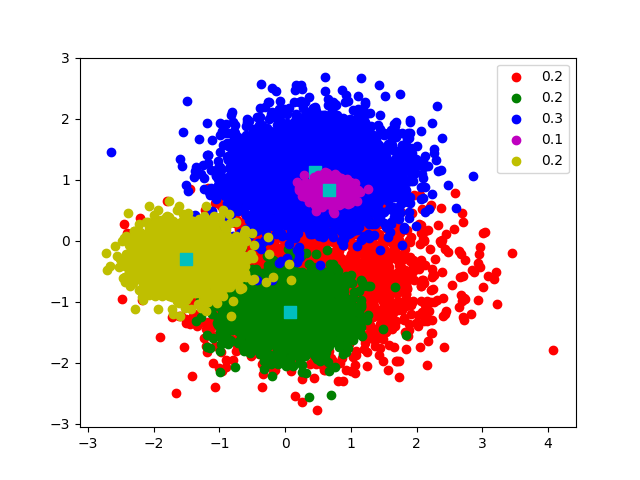
\includegraphics[width=\textwidth]{imgs/kmeans_100D.png}
        \caption{K = 5, 100D, Kmeans}
        \label{kmeans_100D}
    \end{subfigure}
    \begin{subfigure}[b]{0.45\textwidth}
        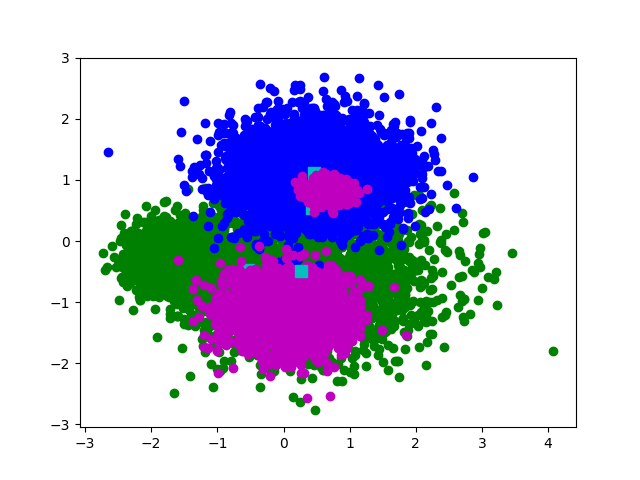
\includegraphics[width=\textwidth]{imgs/GMM_100D.png}
        \caption{K = 5, 100D, GMM}
        \label{GMM_100D}
    \end{subfigure}
\end{figure}

\section{Discover Latent Dimensions}

\subsection{Factor Analysis}

1, [2 pt.] 
First, we have,
\begin{align}
P(\mathbf{x}) & = \int_{\mathbf{z}}  P(\mathbf{x} | \mathbf{z}) P(\mathbf{z}) d\mathbf{z}
\end{align}
From the multivariate results appended in the assignment, we have,
\begin{align}
P(\mathbf{z}) & = \mathcal{N}(\mathbf{z} | 0, I) \nonumber \\
P(\mathbf{x} | \mathbf{z}) & = \mathcal{N}(z | W \mathbf{z} + \bm{\mu}, \Psi) \nonumber \\
P(\mathbf{x}) & = \mathcal{N}(\mathbf{x} | \bm{\mu}, \Psi + W W^{\top} ) 
\end{align}

2, [3 pt.] The training, validation and testing marginal likelihoods are $8399.542$, $1238.54980469$ and $4644.74414062$ respectively. The visualization of weights are in Fig. \ref{FA_weight_1} - \ref{FA_weight_4}. You can see that the weight capture the some parts of digits. For example, Fig. \ref{FA_weight_1} and \ref{FA_weight_3} captures the shape of ``5" and Fig. \ref{FA_weight_2} and \ref{FA_weight_4} captures ``3".

\begin{figure}
    \centering
    \begin{subfigure}[b]{0.24\textwidth}
        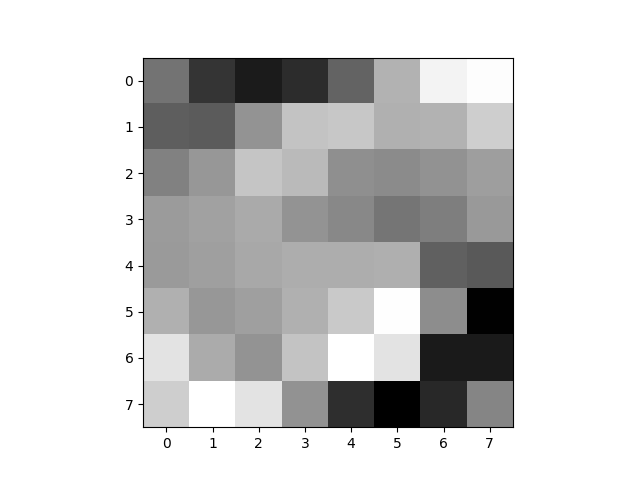
\includegraphics[width=\textwidth]{imgs/FA_weight_1.png}
        \caption{Weight 1}
        \label{FA_weight_1}
    \end{subfigure}
    \begin{subfigure}[b]{0.24\textwidth}
        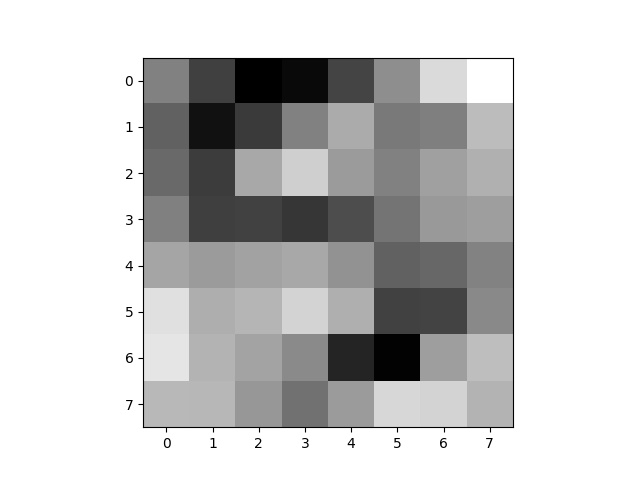
\includegraphics[width=\textwidth]{imgs/FA_weight_2.png}
        \caption{Weight 2}
        \label{FA_weight_2}
    \end{subfigure}
    \begin{subfigure}[b]{0.24\textwidth}
        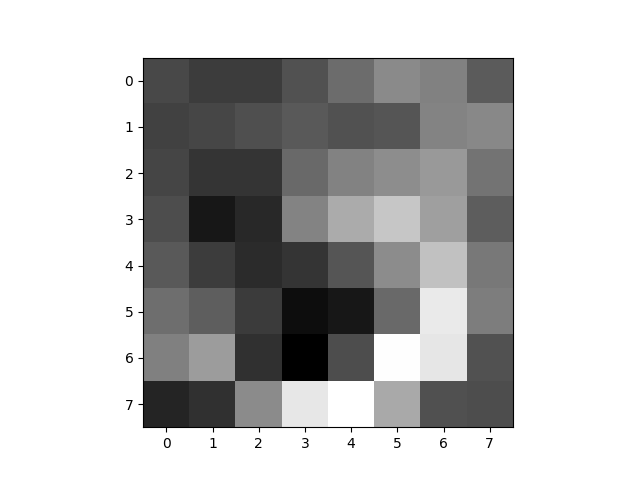
\includegraphics[width=\textwidth]{imgs/FA_weight_3.png}
        \caption{Weight 3}
        \label{FA_weight_3}
    \end{subfigure}
    \begin{subfigure}[b]{0.24\textwidth}
        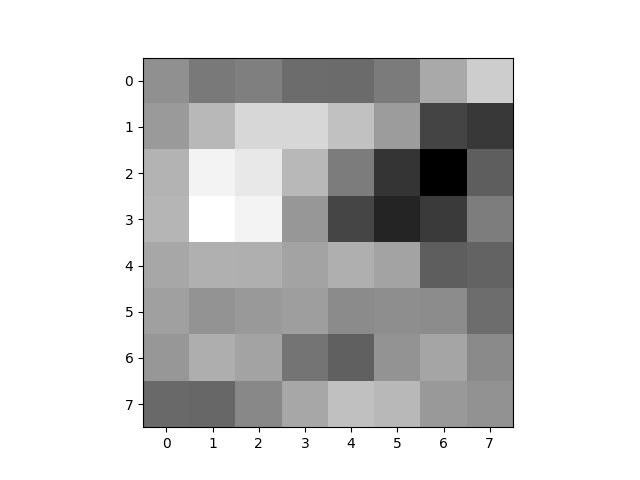
\includegraphics[width=\textwidth]{imgs/FA_weight_4.png}
        \caption{Weight 4}
        \label{FA_weight_4}
    \end{subfigure}    
\end{figure}

3, [3 pt.]

The first component of PCA is $[-2.72359396e^{-04}, -2.61620560e^{-04}, 9.99999929e^{-01}]$ which approximately corresponds to the maximum variance direction, i.e., $x_3$.

The conditional distribution of $\mathbf{s}$ (posterior) of a new data point $\mathbf{x}^*$ in a FA is:
 $p(\mathbf{s} | \mathbf{x}^*) = \mathcal{N}\big(\mathbb{s}; \Sigma W^T\Psi^{-1}(\mathbf{x}^* - \boldsymbol{\mu}), \Sigma\big)$ (Eq(4) of Multivariate Gaussian Results) where $\Sigma = (I + W^T\Psi^{-1}W)^{-1}$. Now let us definite $W_{proj} \triangleq \Sigma W^T\Psi^{-1} = (I + W^T\Psi^{-1}W)^{-1}W^T\Psi^{-1}$. Therefore, $W_{proj}$ is the ``principle component'' matrix that transforms the observation data to the latent space of FA instead of the $W$ matrix. 
 
The first component of $W_{proj}$ is $[3.48705414e-01,   5.76612226e-01,  4.26386575e-08]$ which is the maximum correlation direction, i.e. $x_1+x_2$

\end{document}

